\chapter{Literature Review}
\section{Brush-less DC motor driving}
\subsection{Brush-less DC motor}
Most UAV platforms spin their propellers using Brushless-DC (BLDC) motors due to their low weight, high top speeds and efficiency. Therefore, it is  imperative to know the basic principles to analyze ESCs. 

A BLDC motor can be 1, 2 or 3-phase. However, the most efficient version at high speeds and the ones used for UAVs is the 3-phase version. Therefore, the BLDC term will refer to 3-phase BLDC motors. Figure \ref{fig:bldcm} shows a simplified diagram with only 4 magnetic poles whereas a typical motor used for UAVs would have 14. Here,the stator includes coils and the rotor has permanent magnets.

\begin{figure}
    \centering
    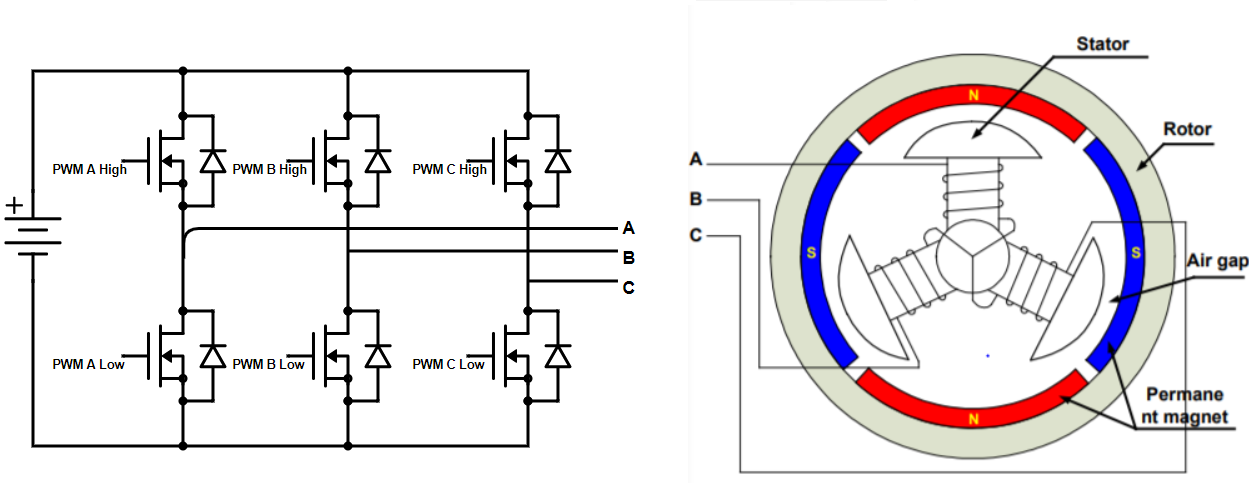
\includegraphics[width=\textwidth]{images/bldcm_diagram.png}
    \caption{\textit{Left} MOSFET bridge driver. \textit{Right} BLDC motor simplified \cite{Zhao_BLDCFundamentals}}
    \label{fig:bldcm}
\end{figure}

\subsection{BLDC motor driving methods}
\label{sec:bldc_driving_methods}
Two configurations can be used to run BLDC motors as mentioned in \cite{Mogensen_ESC_Motor_Control2016}, both based on Pulse Width Modulation (PWM). These are Trapezoidal and Sinusoidal. They differ in the ideal driving voltage wave-forms to use when driving the motor coils. In both cases, the best performing phase shift between phases is 120\textdegree.  The effective instantaneous voltage in each coil is a fraction of the DC power supply. PWM approximates this fraction by providing a pulsing signal with a corresponding duty cycle (fraction of time the signal is high). 
To generate these PWM signals from a DC power source, power MOSFETs are used in bridge configurations. The specific configuration used for BLDC motors is shown in Figure \ref{fig:bldcm}
\newline

\textit{Trapezoidal:}
Here the ideal driving waveform is a trapezoidal wave. As shown in Figure \ref{fig:foc_trapezoidal_signals} bottom. This method is easier to implement in hardware since a relatively low accuracy in rotor angular position estimation is needed. However, there are significant power loses caused by many spikes in the signal and also because the electrical magnetic field caused by the stator is only instantaneously at the optimal orientation relative to the rotor magnetic field (perpendicular). Here, the duty cycle put through the active phases is constant for the same rotor speed
\newline

\textit{Sinusoidal:}
In this case, the ideal driving waveform is a sinusoid as seen in figure \ref{fig:foc_trapezoidal_signals} top. Note that for the same rotor speed, the duty cycle continuously changes over an electrical period to mimic the ideal sinewave. This is because of the waveform continuously changing and because feedback control \footnote{This is not rotor speed control} is used to maintain the relative orientation rotor-startor magnetic field orientation optimal (90\textdegree). Since the duty cycle is changed more often and depending on the rotor position, this method requires a significantly higher accuracy in rotor angular position estimation.
Higher efficiency is obtained in two fronts:less pulsing implies less spikes and therefore switching power losses; the magnetic fields relative orientation is controlled to be optimal. 

\begin{figure}
    \centering
    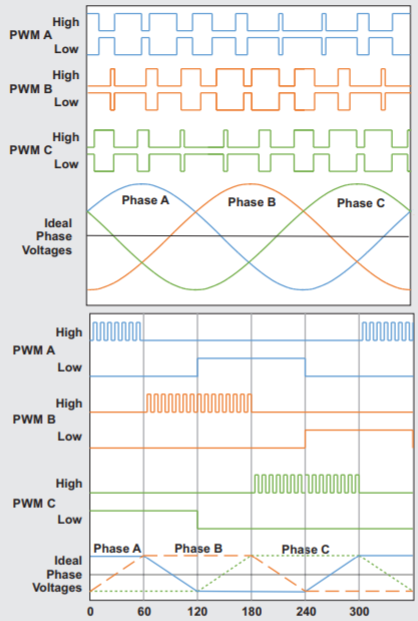
\includegraphics[width=0.5\textwidth]{images/foc_trap_sig.png}
    \caption{PWM Phase signals vs Rotor Position. \textit{Top} Sinusoidal FOC, \textit{Bottom} Trapezoidal. Adapted from \cite{Mogensen_ESC_Motor_Control2016}}
    \label{fig:foc_trapezoidal_signals}
\end{figure}


\section{Electronic Speed Controllers}
\subsection{General structure}
The circuits that run the BLDC motors are commonly known as Electronic Speed Controllers (ESC). However, the majority of current available ones do not perform direct motor speed control. Their core components are a micro-controller, gate drivers, back Electro-motive foce (EMF) measurement resistors and the MOSFETs (shown in Figure \ref{fig:bldcm}). In essence, what they do is receive a throttle signal from a Flight Controller (FC) representing the amplitude of the ideal driving signal (explained in previous subsection, Fig. \ref{fig:foc_trapezoidal_signals}). The diagram in Figure \ref{fig:esc_diag} shows a general electrical architecture of ESCs. Note that gate drivers are simply interface circuits that allow to turn on/off the MOSFETs.
\begin{figure}
    \centering
    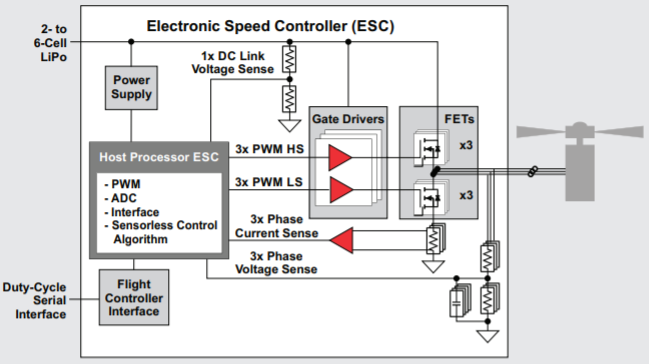
\includegraphics[width=0.8\textwidth]{images/esc_diagram.PNG}
    \caption{ESC general architecture \cite{Mogensen_ESC_Motor_Control2016}}
    \label{fig:esc_diag}
\end{figure}

\subsection{Communications}
ESCs need to communicate with the FC to receive throttle commands and in some cases they also send status messages. Hence, some protocols have been used and other have been developed in the context of UAVs.

\subsubsection{Analog Protocols}
All of these protocols are based on Pulse width modulation given a maximum and a minimum pulse width to be set as maximum and minimum throttle. Hence, these protocols are commonly called RCPWM. Thee different protocols in this category merely differ in the pulse period. Figure \ref{fig:oneshot} depicts these kind of signals on the top and Table \ref{tab:tab_esc_prot}  shows their transmission parameters.

\begin{figure}
    \centering
    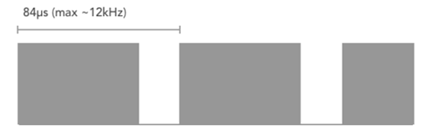
\includegraphics[width=0.8\textwidth]{images/oneshot_sketch.png}
    \caption{Oneshot protocol \cite{BackyardRobotics2018}}
    \label{fig:oneshot}
\end{figure}

\begin{table}
\begin{center}
 \caption{ESC protocols' speeds}\vspace{1ex}
 \label{tab:tab_esc_prot}
 \begin{tabular}{l|rrr}
 \hline
Protocol & Type & Pulse width range [$\mu s$]  & Max Update Rate [kHz] \\ \hline \hline
PWM                 & Analog & 1000 - 2000      & 2000\\
Oneshot125          & Analog & 125 - 250        & 250\\
Oneshot42           & Analog & 42 - 84          & 84\\
Multishot           & Analog & 5 - 25           & 40\\
Dshot150            & Digital & 2.5, 5$^*$          & 9\\
Dshot300            & Digital & 1.25, 2.5$^*$       & 18\\
Dshot600            & Digital & 0.625, 1.25$^*$     & 37\\
Dshot1200           & Digital & 0.312, 0.625$^*$    & 75\\
Bidirectional Dshot & Digital & Same as Dshot   & Same as Dshot \\
Proshot             & Digital & Same as Dshot   & Same as Dshot\\
UAVCAN              & Digital & NA              & NA\\
 \end{tabular}
\end{center}
\footnotesize{$^*$ Pulses can only take either of the two values (Digital)}
\end{table}



\subsubsection{Digital Protocols} \label{sec: esc_dig_prot}
Even though most of these protocols are widely known as digital, the true purely digital protocol is UAVCAN. The rest define certain specific pulse time durations to high or low. Dshot will be explained thoroughly in particular given that it's the basis of all the other methods but UAVCAN.
\newline
\textit{Dshot: } This method consists of a 16-bit packet streamed continuously. Each bit is encoded as a pulse with one of to widths, depending on the pulse width version. Figure \ref{fig:dshot} shows the typical DShot signal and the information organization in each packet. The packet is divided into three sections: 
\begin{itemize}
    \item Throttle command: Consists of 11 bits (Decimal values 0 -2047). Commands in the range [0,47] are status request commands whereas values in the range [48,2047] encode a 2000 levels throttle command.
    \item Telemetry request: When this bit is high, telemetry is hight, the ESC is sends a telemetry information packet from the to the FC. Including information such as: Motor Electrical RPM, ESC Temperature, Supply Voltage, Current (Available only in certain ESCs). This telemetry message is sent via another pin using Universal Asynchronous Receiver/Transmitter protocol (UART) at 115200 baudrate.
    \item Cyclic Redundancy Check (CRC): Used to check for data corruption during transmission.
\end{itemize}

\begin{figure}
    \centering
    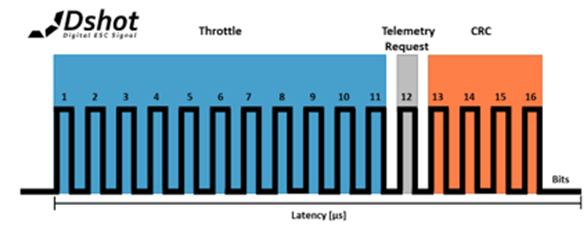
\includegraphics[width=0.8\textwidth]{images/dshot_sketch.png}
    \caption{Dshot Signal Structure \cite{Speedgoat2020}}
    \label{fig:dshot}
\end{figure}

\textit{Bidirectional Dshot:} This protocol uses exactly the same signal from the ESC to the FC. The difference is the medium of transfer for the Telemetry signal. In this case, the telemetry packet is sent to the FC through the same throttle pin.
\newline

\textit{Proshot: } The data side of this protocol works the same way as Dshot. The 16 bit digital signal is set as a 4 pulse train where each pulse can encode 4 pulse widths (as opposed to only 2 in Dshot).
\newline

\textit{UAVCAN: } As its name suggests, this a full level software platform based on the Controller Area Network (CAN) bus. It supports two-way communication between multiple agents over a twisted pair wire. The signals sent are merely digital (Only high and low voltages at same duration). The protocol packet convention is illustrated in Figure \ref{fig:canbus}. Where the elements are explained in \cite{Corrigan2016} as:
\begin{itemize}
    \item SOF (1 bit): Dominant Start of Frame bit. Used for synchronization.
    \item Identifier (11-bits): Establishes message priority.
    \item RTR (1 bit): Remote Transmission Request. Asks next node for transmission.
    \item IDE (1 bit): Identifies if standard CAN is used or not.
    \item r0 (1 bit): Reserved.
    \item DLC (4 bits): Data length. Number of bytes transmitted.
    \item Data (1-64 bits): Actual data transmitted.
    \item CRC (16 bits): Cyclic redundancy check.
    \item ACK (1 bit): Indicates error free reception.
    \item EOF (7 bits): Indicates end of packet.
    \item IFS (7 bits): Time required to buffer data.
\end{itemize}

Hence, communication in this protocol is very reliable on the expense of having to send many extra bits for agent coordination and error checking. The maximum bitrate allowed in this protocol is $1Mbit/s$. However, its data transfer rate is decreased by the number of agents connected together and the amount of data each sends. If only one ESC was connected with the FC, the absolute maximum theoretical data rate would be 4.3kHz. Another problem that could arise when using this protocol is significant delays between each rotor command especially between the first motor and the last motor to receive commands. This is because each agent needs to queue when receiving and sending messages as the bus is shared.

\begin{figure}
    \centering
    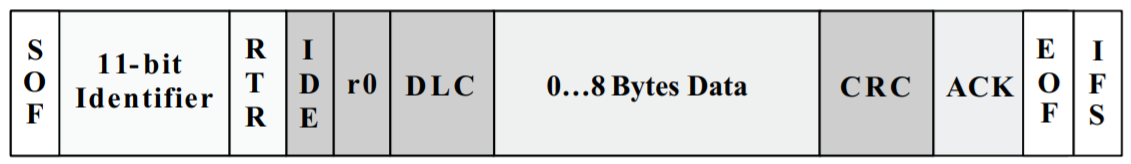
\includegraphics[width=0.9\textwidth]{images/canbus_sketch.png}
    \caption{CAN bus protocol \cite{Corrigan2016}}
    \label{fig:canbus}
\end{figure}

\section{Related Work on ESCs characterization}

There have been some studies regarding modeling and characterization BLDC motors driving hardware, given the popularity of their use in UAVs in the last decade. There have been studies in both efficiency and estimation modeling for their dynamic behavior. 
\subsection{Efficiency}
Regarding efficiency estimation, several power loss models have been developed based on non-ideal electronic components in the ESCs. Indeed, \cite{Gong2017,Gong2018} propose linear and non-linear models for ESC efficiency. There, it is shown that the efficiency changes depending on voltage powering the ESC and current provided to the motor.  Furthermore, \cite{Millett2012, Keskar} define complete models of power loss calculation for ESCs driving BLDC motors and \cite{Graovac2006} models MOSFET power losses. These factors were accounted for in a more generalized model described in \cite{Tritium2013} and summarized in Equation \ref{eq:power_loss}.

\begin{equation}
  P_{loss}=R_{eq}I_o^2+(\alpha I_o+\beta)V_{bus}+Cf_{eq}V_{bus}^2\, .
    \label{eq:power_loss}
\end{equation}

In this equation, $R_{eq}$ represents the MOSFET on resistance usually given in data-sheets, $I_o$ the output current, $V_bus$ the battery voltage, $\alpha$ and $\beta$ are model values and $Cf_{eq}$ is the equivalent capacitance frequency product for overall circuit.

\subsection{Modeling for Control}
Another stream of research is dedicated to determine the input-output characteristics of ESC-BLDC motor behavior. 
\newline

Direct Throttle to Thrust mapping is subject of investigation by many sources. A linear first order differential relationship about operating points is proposed by \cite{Yoon2015}, with only two determined parameters: gain and time constant. This model was further improved by \cite{Torres2020} by introducing a dead-time parameter to account for communication delays and buffer timing which makes it non-linear.
Supply Voltage is show as another parameter that affects ESC-Throttle mapping in \cite{Szafranski2014} where they define a linear MIMO representation with voltage and throttle as inputs; and current and thrust as output, including non-linear elements.
\newline

Other studies have instead focused on the Throttle - rotor speed correspondence. In this category, \cite{Prakosa2019} encountered non-linear steady state mapping. Furthermore, one of the first models that incorporated voltage is given by \cite{Moutinho2015} where the steady state value is defined rotor speed is defined as proportional to the voltage and a first order polynomial of the throttle value, and the dynamics still as a first order differential function, these relationships are detailed in Equations \ref{eq:rpm_V_throt}.

\begin{equation}
 \frac{\omega}{V}= at +b  \quad and \quad \frac{\omega /V}{t}=\frac{k}{\tau s+1}\, .
 \label{eq:rpm_V_throt}   
\end{equation}

Where $a$ and $b$ are linear fit parameters based on linear fit of steady state data, $k$ and $\tau$ are gain and time constant. $\omega$ represents rotor speed, $V$ battery voltage and $t$ throttle signal.
\newline

Another stream of investigation in this area focused on frequency methods to identify the responses to throttle commands. Chirp sinusoid input throttle signals are used in \cite{Xiang2015} and the rotor speed output is analyzed. They define a first order differential relation for the ESC output voltage and the utilize a sophisticated motor model to transfer as a transfer function between effective voltage on the motor and rotor speed. Their model even includes cogging modeling, specially important at low speeds. Their complete model is third order differential.
Besides, \cite{Wu2018} uses steady state response and frequency response using staircase and sinusoidal chirp input throttle signals, but analyses the thrust and torque generated. The model is semi-empirical and includes non-linearities such as torque friction, drag and rotor inertia. However, it assumes a PI loop in the ESC to purpose a model, which is not always the case.

The last stream of investigation in this domain, was merely as data analysis. This includes \cite{Kotarski2017} who analyzed thrust, rotor speed and power outputs, which where presented graphically. Additionally \cite{Sulewski2018} also shows graphical representations of efficiency, power, current, voltage, thrust and torque for different thrust inputs.